\chapter{Softvér}
V našej práci je cieľom implementácie matematicky odvodených konceptov vizualizácia vypočítaných plôch. Pri vytváraní plôch nám napadlo vytlačiť si niekoľko modelov v 3D tlačiarni. 

V tejto kapitole v prvej časti uvedieme stručnú špecifikáciu softvéru, v druhej časti zdôvodnime výber programovacieho jazyka a knižníc, opíšeme proces ich inštalácie, zdôvodnime použité programovacie prostredie a uvedieme jeho konfiguráciu pre naše použitie. V tretej časti uvedieme beh skriptov a na záver, vo štvrtej časti, krátko opíšeme proces 3D tlače plôch. Všetky vytvorené skripty, vymodelované plochy, súbory pripravené na 3D tlač a ďalšie súbory sa nachádzajú na GitHube v repozitári \url{https://github.com/tutka13/Masters-Thesis}.
 
\section{Špecifikácia}
Hlavným cieľom je vytvorenie 3D plochy - obálky sfér a elipsoidov, kde používateľ zadá vstupné parametre. Softvér vypočíta a vymodeluje plochu podľa procesu.

\subsection{Vstup}
\textbf{Obálka sfér:}

Parametrizácia priestorovej krivky $m(t)$ stredov sfér, funkcia polomeru $r(t)$, interval $I$ vykreslenia plochy parametra $t$, vzorkovanie plochy, teda krok vyčíslenia a posun plochy v priestore.

\noindent \textbf{Obálka elipsoidov:}

Parametrizácia priestorovej krivky $m(t)$ stredov elipsoidov, konštanty $a$ a $b$, interval $I$ vykreslenia plochy parametra $t$ a vzorkovanie plochy, teda krok vyčíslenia a posun plochy v priestore.
\subsection{Výstup} 
\textbf{Obálka sfér:}

Vizualizácia troch ploch - jednoparametrického systému sfér, jednoparametrického systému charakteristických kružníc a výslednej plochy - obálky sfér.

\noindent \textbf{Obálka elipsoidov:}

Vizualizácia troch plôch - jednoparametrického systému elipsoidov, jednoparametrického systému charakteristických kriviek, výslednej plochy - obálky elipsoidov.

\subsection{Postup práce}
Priebeh procesu je v oboch prípadoch, pre sféry a elipsoidy, rovnaký.
Najprv vymažeme všetky objekty zo scény. Po prečítaní vstupných parametrov z textového súboru sa prevedú symbolické výpočty. Vytvoríme si prázdne zoznamy, do ktorých sa v ďalšom kroku ukladajú numericky vyčíslené hodnoty symbolických výrazov. Plochy sa vykresľujú po jednotlivých objektoch. Objekt je kružnica sféra alebo elipsoid. Pri vykresľovaní objektov prechádzame zoznamy jeho uložených parametrov. Po vykreslení daného objektu zrealizujeme jeho posun a natočenie v priestore. Ak boli objekty kružnice, vhodne ich pospájame a vhodne medzi ne doplníme pletivo \textit{(mesh)}. Na záver scénu uložíme.
%\begin{itemize}
%	\item vymazanie scény
%    \item čítanie parametrov z textového súboru
%    \item symbolické výpočty
%    \item vytvorenie prázdnych polí
%    \item numerické vyčíslenie symbolických výrazov
%    \item uloženie hodnôt do poľa
%    \item určenie normál charakteristických kružníc
%    \item označenie charakteristických kružníc
%    \item interpolácia medzi dvoma charakteristickými kružnicami
%    \item posun plôch v priestore
%    \item vizualizácia plôch
%    \item uloženie scény do databázy
%\end{itemize}

%\begin{itemize}
%	\item čítanie parametrov
%    \item natočenie a posun elipsoidov
%    \item určenie parametrov škálovania
%    \item umiestnenie elipsodiu do každého bodu krivky $m(t)$
%    \item derivácia jednoparametrického systému plôch 
%    \item extrahovanie koeficientov
%    \item určenie typu plochy
%    \item nahradenie elipsoidov zodpovedajúcimi kružnicami
%    \item výpočet natočenia kružníc
%    \item vizualizácia plochy
%    \item uloženie plochy do databázy
%\end{itemize}
\subsection{Funkčnosť softvéru} 
Potrebné dátové štruktúry:
\begin{itemize}
	\item zoznam
\end{itemize}
Potrebné funkcie:
\begin{itemize}
	\item vymazanie objektov zo scény 
    \item čítanie parametrov z textového súboru
    \item symbolické výpočty
    \item numerické vyčíslenie
    \item posun objektu v priestore
    \item interpolácia - doplnenie pletiva medzi dvomi charakteristickými kružnicami
    \item uloženie scény do databázy
\end{itemize}
\section{Výber softvéru a jeho inštalácia}
Na výpočet a vizualizáciu plôch sme sa rozhodli využiť kombináciu Blenderu a jazyka Python. Python je momentálne jedným z najpopulárnejších a najpoužívanejších programovacích jazykov, s knižnicami vhodnými pre matematické výpočty. Okrem toho dokáže generovať výstupy vo formáte \LaTeX. Je užívateľsky intuitívny. Blender je významným nástrojom pre prácu s 3D grafikou. Vzhľadom na trojrozmernú povahu našich plôch, nám jeho použitie umožnilo vytlačiť aj niekoľko fyzických modelov v 3D tlačiarni.
\subsection{Blender}
Blender je open source balík na tvorbu 3D. Podporuje celú 3D technológiu - modelovanie, rigging, animáciu, simuláciu, renderovanie, kompozíciu a sledovanie pohybu, dokonca aj strih videa a tvorbu hier. Pokročilí používatelia využívajú rozhranie API programu Blender pre skriptovanie v jazyku Python na prispôsobenie aplikácie a písanie špecializovaných nástrojov \cite{Blender}. Pre účely tejto práce sme využili Blender 4.0.2, stiahnuteľný na webstránke \cite{BlenderDownload}. Blender umožňuje rozšírenie svojej funkcionality pomocou skriptovacieho jazyka Python, ktorý je integrovaný priamo do softvéru, teda nie je potreba samostatnej inštalácie. Okrem toho Blender obsahuje špeciálnu knižnicu bpy, ktorá slúži na vykonávanie príkazov v Blenderi. Na vytváranie skriptov slúži prostredie Scripting, ktoré obsahuje okná na písanie, úpravu textu a Python konzolu. Je možné pracovať aj v externom programovacom prostredí \cite{BlenderAPI}.

\begin{figure}[h]
	\centering
	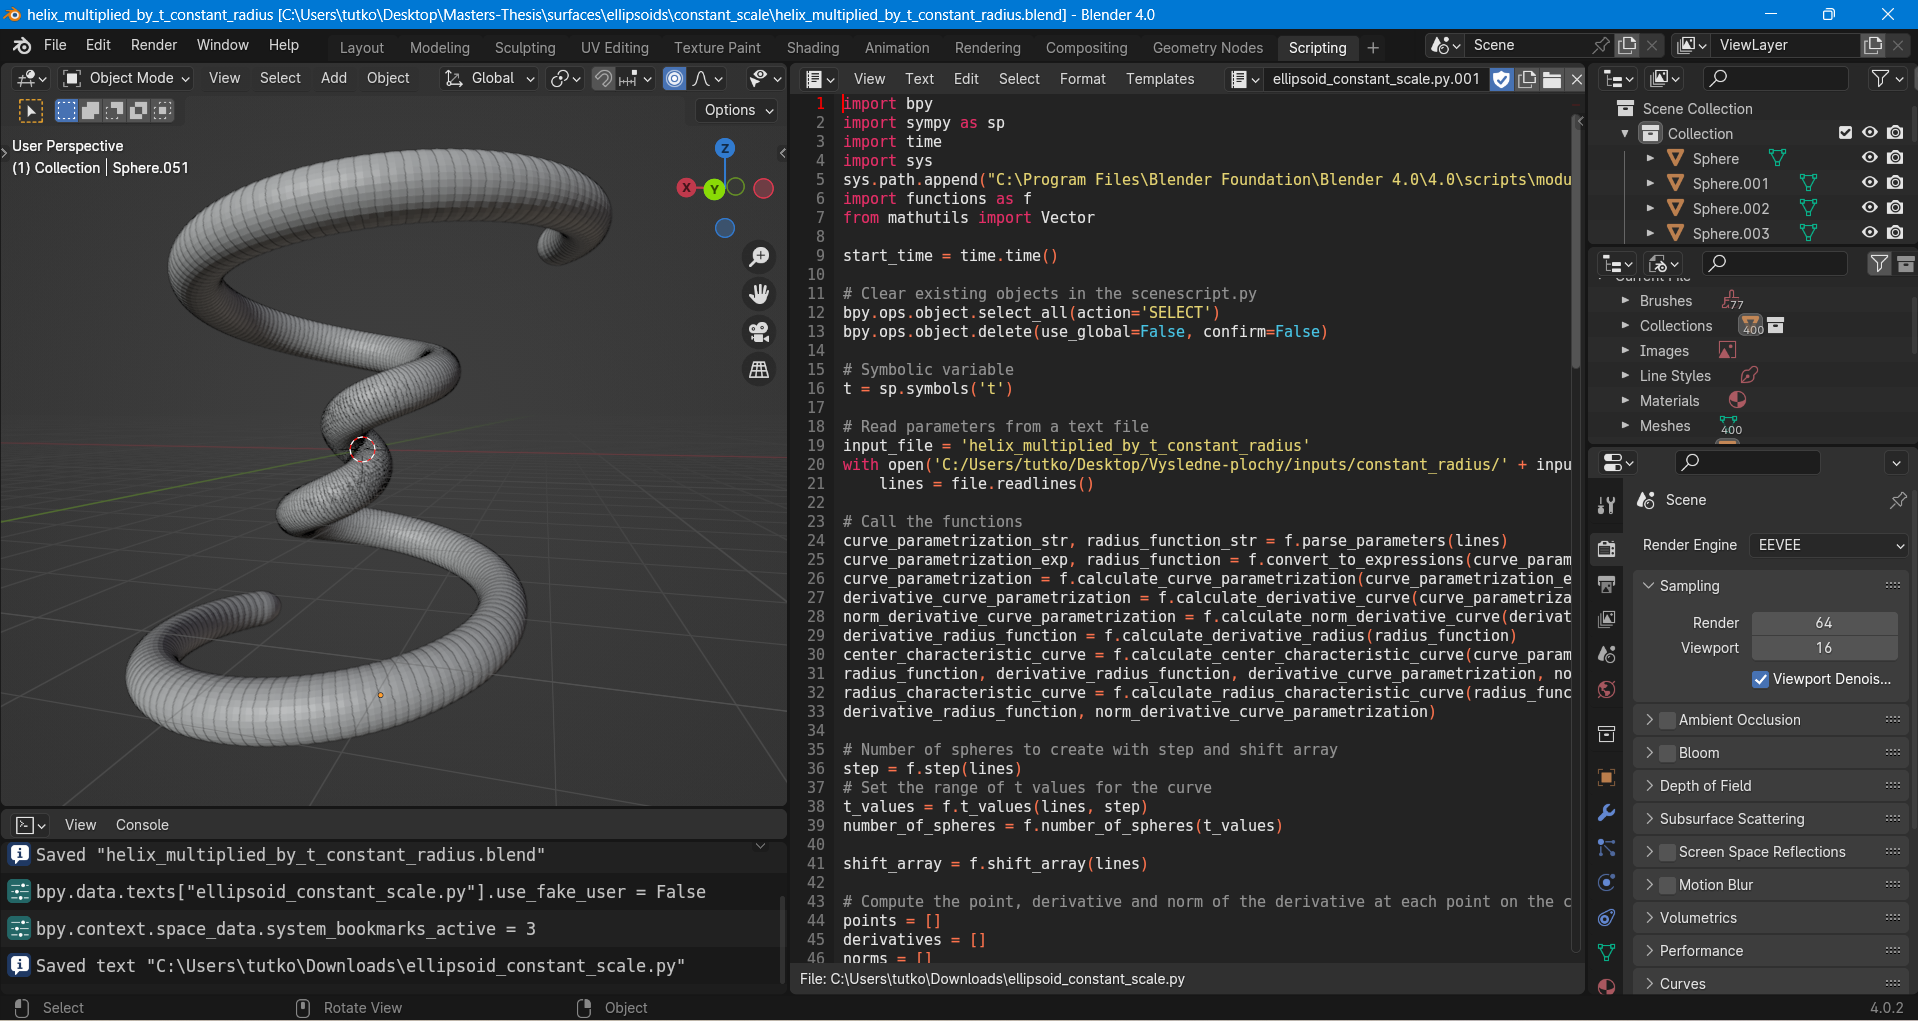
\includegraphics[width=\textwidth]{images/blender.png}
	\caption[Softvér Blender.]{Plocha vygenerovaná skriptom v Blendri.}
	\label{fig:blender}
\end{figure}

\subsection{Python}
Python je vysokoúrovňový programovací jazyk, ktorý je populárny pre svoju jednoduchosť a čitateľnosť syntaxe. Má široké využitie v rôznych odvetviach, ako sú web development, vedecké výpočty, umelá inteligencia, automatizácia, spracovanie dát a mnoho ďalších. Pri používaní priamo v Blendri nie je potrebná inštalácia. Pri otvorení prostredia Scripting v Blendri sa vľavo v konzole nachádza informácia o verzii Pythonu, ktorú Blender používa. V našom prípade je to 3.10.13.
\subsection{Knižnice}
Na výpočet a zobrazenie plôch v Blendri sme využili nasledovné knižnice
\begin{itemize}
\item bpy: knižnica Blenderu, ktorá umožňuje manipuláciu s objektmi v Blendri pomocou príkazov vytvorených v skriptoch,
\item math: základné matematické funkcie a konštanty pre numerické výpočty, obsahuje funkcie ako $\sin, \cos, \log$ a ďalšie, ako aj konštanty ako $\pi$ a $e$,
\item mathutils: je súčasťou Blenderu a poskytuje množstvo matematických funkcií a nástrojov pre prácu s 3D objektami, obsahuje funkcie na rotácie, transformácie, výpočet normál a ďalšie operácie v 3D priestore,
\item matplotlib.pyplot: rozhranie na tvorbu vizualizácií a grafického zobrazenia dát, tvorbu grafov, histogramov, kontúrových máp a ďalších typov vizuálnych reprezentácií dát,
%1.26.0 numpy
\item numpy: nástroje na manipuláciu s vektormi, maticami, poliami a ďalšími objektami potrebnými pre zložitejšie výpočty 
\item sympy: nástroje na symbolické výpočty, algebraické manipulácie, riešenie rovníc a ďalšie matematické operácie potrebné pre pokročilé výpočty,
\item sys: prístup k niektorým systémovým špecifikáciám a funkciám, medzi jej použitia patrí prístup k argumentom príkazového riadku, manipulácia s cestami k súborom a niektoré informácie o systéme, ako verzia Pythonu,
\item time: získanie času v milisekundách. 
\end{itemize}
\subsubsection{Inštalácia knižníc}
Pip je inštalátor balíkov pre Python, ktorý spravuje knižnice pre jazyk Python. Používa sa na inštaláciu z Python Package Index. PyPI je knižníc pre programovací jazyk Python. Keďže sme Python stiahli z oficiálnej stránky Python \cite{PythonDownload}, pip sa inštaloval automaticky \cite{Pip}. Overiť, či máme naištalovaný pip, možno pomocou príkazového riadku, ktorý otvoríme vyhľadaním cmd v ponuke vyhľadávania a zadaním
\verb|python -m pip --version.|
V našom prípade pracujeme s verziou pip 24.0. Následne je možné inštalovať všetky potrebné knižnice v príkazovom riadku zadaním \verb|pip install názov knižnice.|
\subsection{Programovacie prostredie}
Keďže prostredie Scripting v Blendri nedisponuje mnohými vlastnosťami, ktoré by sme na zjednodušenie tvorby skriptov potrebovali, využijeme externé programovacie prostredie, a to Visual Studio Code. 
\subsubsection{Visual Studio Code}
Na úpravu skriptov pre Python a Python-Blender sme využili programovacie prostredie Visual Studio Code vo verzii 1.82.2, ktorý disponuje farebným zvýrazňovaním kódu, súčasným zobrazením viacerých skriptov, zobrazením súborov v priečinku, kontrolou chýb, ladením programu a ďalšími funkciami. Má intuitívny a prehľadný dizajn, no jeho najväčšou výhodou je množstvo rozšírení, z ktorých je pre prepojenie programov Python a Blender potrebné Blender Development. Toto rozšírenie slúži na ladenie skriptov, ktoré sa spúšťajú v prostredí Blenderu.

\begin{figure}[h]
	\centering
	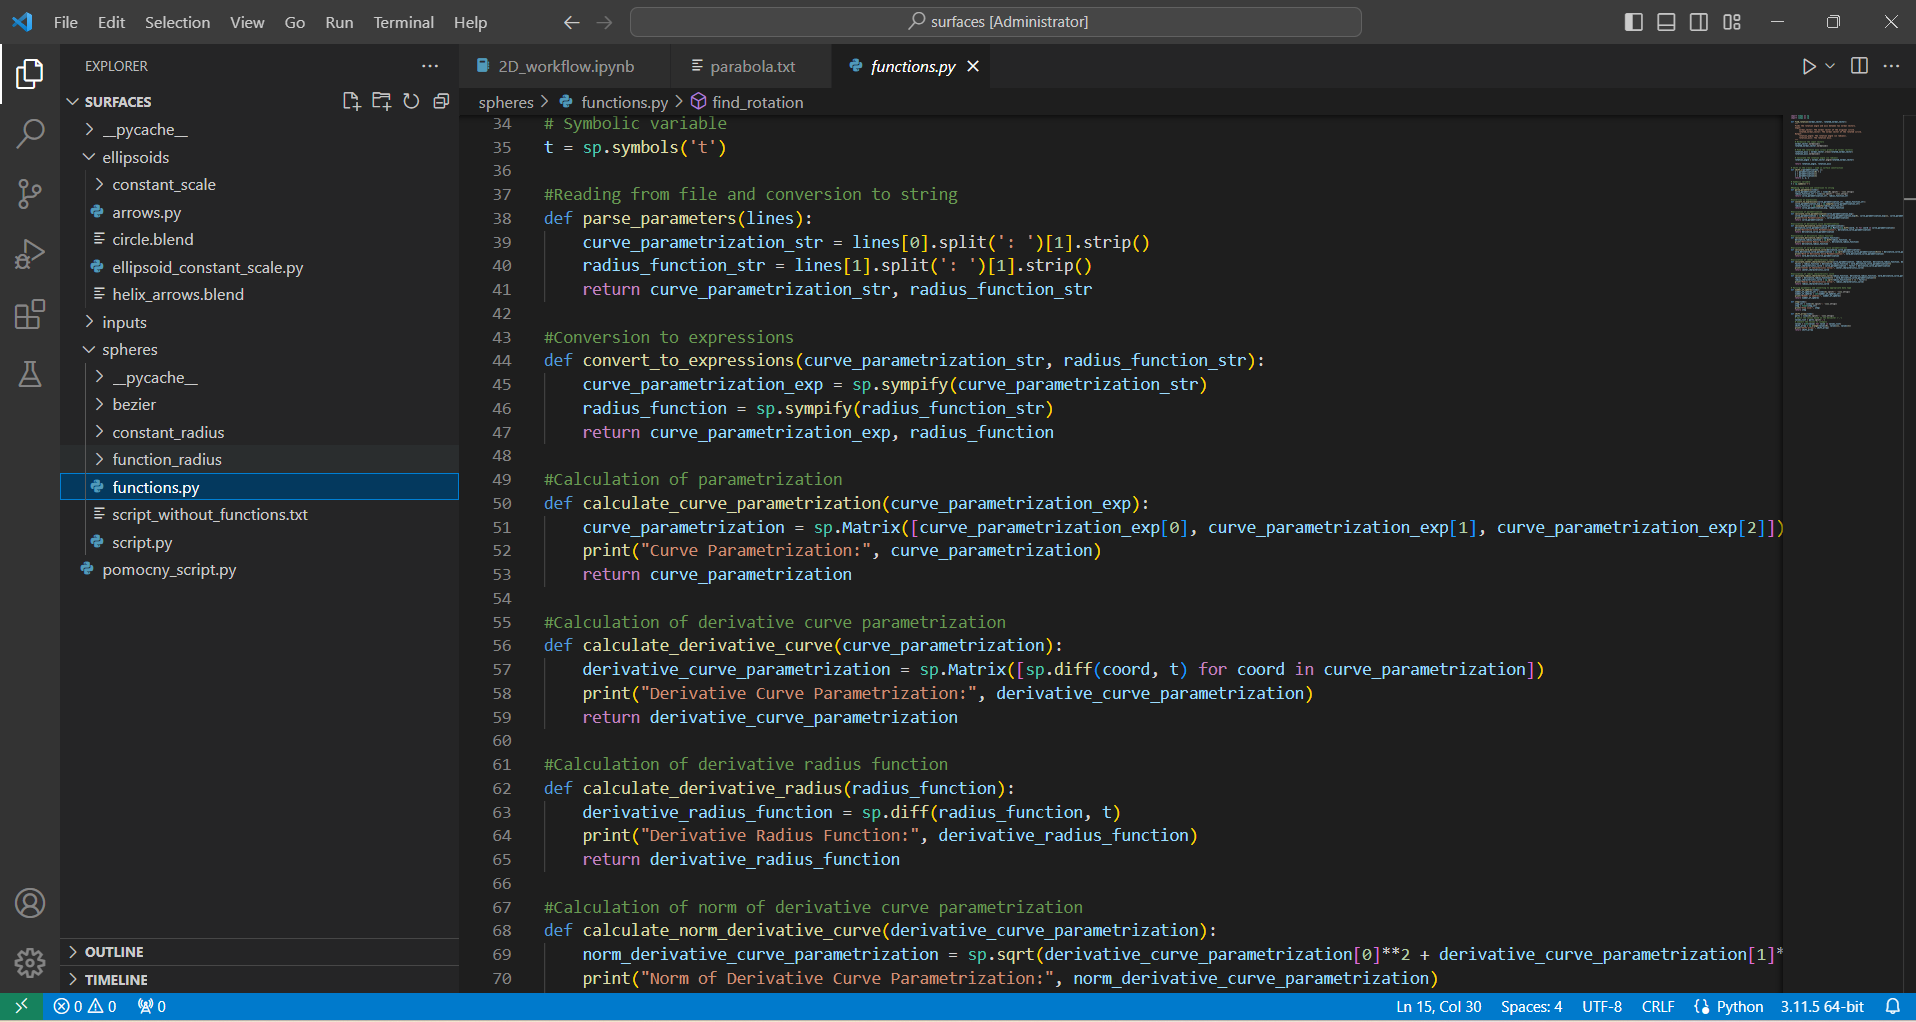
\includegraphics[width=\textwidth]{images/vscode.png}
	\caption[Softvér Visual Studio Code.]{Skipt funkcií pre obálku sfér a elipsoidov vo VS Code.}
	\label{fig:vscode}
\end{figure}

\subsubsection{Konfigurácia VS Code - Python - Blender}
Pre systém Windows sme nainštalovali samostatnú verziu Pythonu \cite{PythonDownload}. Keďže Blender používa Python verziu 3.10.13, mohli sme stiahnuť akúkoľvek vyššiu. Používame verziu 3.11.5. Pri inštalácii je potrebné odkliknúť možnosť \verb|Add Python| \verb|Executable to the path|. Zo stránky \cite{VSCode} sme stiahli VS Code, ktorý sme následne inštalovali. Vo VS Code sme v paneli rozšírení na ľavej strane vyhľadali rozšírenie Python, ktoré vytvorila spoločnosť Microsoft a aj to sme inštalovali. Tým sa umožnila práca VS Code s jazykom Python. Pre používateľsky príjemnejšie používanie knižnice bpy v skriptoch bolo potrebné nainštalovať falošný bpy modul \cite{Fake-bpy-module} príkazom v termináli \verb|pip install fake-bpy-| \verb|module-latest.|
Po dokončení inštalácie sme reštartovali VS Code. V bočnom paneli rozšírení sme vyhľadali Blender development. Po inštalácii sme v priečinku Python v inštalačnom adresári programu Blender otvorili vlastnosti, kartu zabezpečenia a skupinu používateľov \verb|Users|, ktorým sme povolili možnosť \verb|Write|. Vďaka tomuto rozšíreniu sme mohli ladiť program pomocou \verb|Ctrl+Shift+P.| Po stlačení tejto klávesovej skratky sa v hornom paneli zobrazilo kontextové menu, kde sme vybrali \verb|Blender: Build and Start,| čím sme spustili Blender. Proces ladenia programu sme spúšťali možnosťou \verb|Blender:| \verb|Run Script.|
\subsubsection{Jupyter Notebook}
Pre účely našej práce sme potrebovali niekoľko pomocných skriptov na vyčíslenie obálok konkrétnych prípadov v 2D a 3D a na prepis symbolických výpočtov z Maximy do programu \LaTeX. Pri programovaní týchto skriptov sme využívali Jupyter Notebook vo verzii 7.0.4, výpočtový nástroj, pôvodne navrhnutý pre úlohy dátovej vedy, ktorý umožňuje interaktívnu prácu s kódom, rovnicami a vizualizáciami s podporou v 40 programovacích jazykoch. S jeho pomocou je možné vytvárať dokumenty vo formáte JSON, ktoré sú rozdelené do buniek a komunikujú s výpočtovými jadrami cez Interactive Computing Protocol. Jadrá sú zodpovedné za vykonávanie kódu a výstupy. Jupyter Notebook ponúka modulárny dizajn, ktorý umožňuje jednoduché manipulácie s jednotlivými bunkami, vrátane možnosti úpravy bunky bez ďalšieho vplyvu na zvyšnú časť kódu, spätného vrátenia sa a vymazania bunky \cite{Jupyter}. Jupyter Notebook sa nainštaluje rovnako ako Blender Development vo VS Code rozšíreniach. 
%alebo v príkazovom riadku zadaním
%\begin{verbatim}
%pip install jupyterlab
%pip install jupyter notebook.
%\end{verbatim}  
Jednou možnosťou ako spustiť Jupyter Notebook je vytvorenie nového súboru vo VS Code s príponou \verb|Jupyter Notebook .ipynb.| 
\begin{figure}[h]
	\centering
	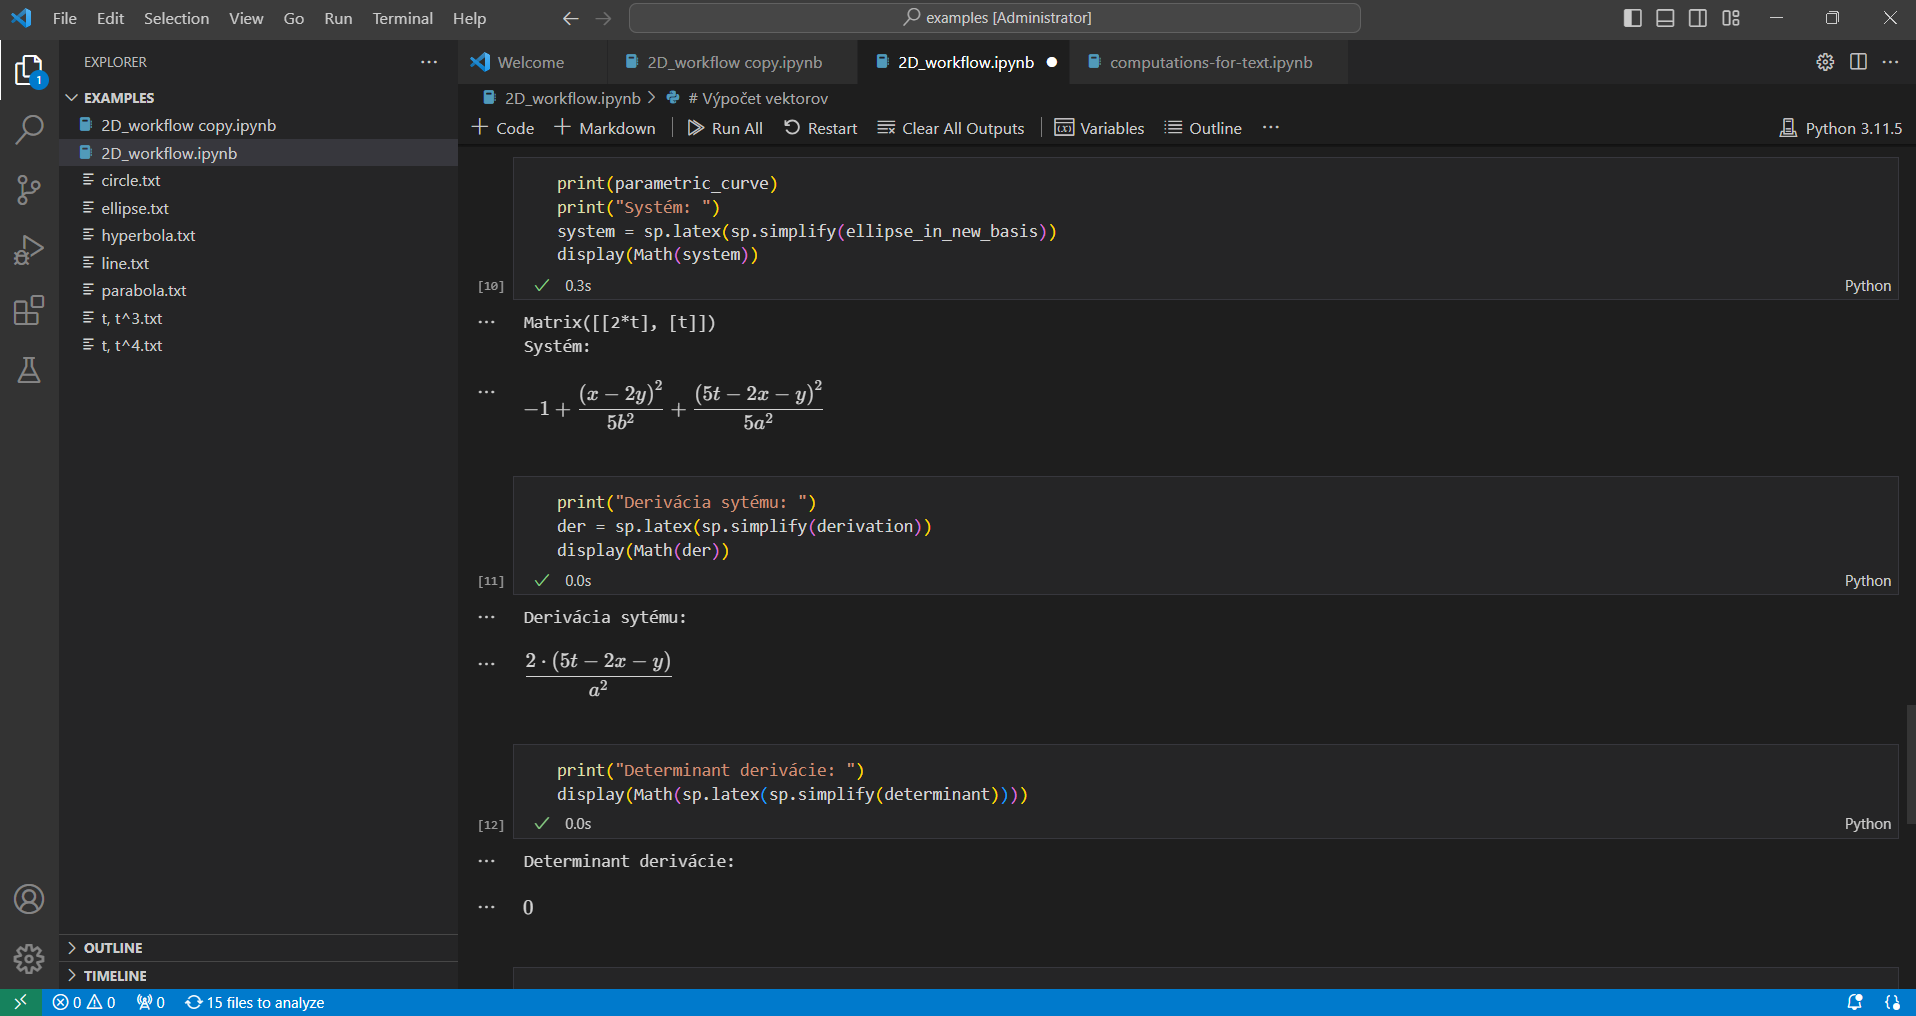
\includegraphics[width=\textwidth]{images/jupyter.png}
	\caption[Jupyter Notebook.]{Výstupy po každej vykonanej bunke v JupyterNotebook.}
	\label{fig:jupyter}
\end{figure}

\section{Implementácia}
V tejto časti sa budeme venovať vývoju skriptov. Skriptov máme niekoľko, no v tejto časti budeme primárne hovoriť o skripte na vymodelovanie obálky sfér \verb|envelope_of_spheres.py|, skripte na vymodelovanie obálky elipsoidov \verb|envelope_of_spheres.py| a o skripte s používanými funkciami \verb|envelope_of_spheres.py|. Všetky výpočty vrátane rotácie kružníc a elipsoidov sú realizované pomocou funkcií definovaných v module \verb|envelopes.py|. Modul sme umiestnili do adresára programu Blender, v ktorom Blender ukladá svoje skripty a moduly. V našom prípade to bolo \verb|C:\Program Files\Blender Foundation\Blender 4.0\4.0\scripts\modules|. Potom sme importovali modul do programu Blender štandardným spôsobom. 
\subsubsection*{Obálka sfér}
Najprv sme začali vyvíjať skript pre obálku sfér, kde bolo hlavnou myšlienkou zostrojenie obálky sfér na intervale $I$ s vhodným vzorkovaním plochy pre parameter $t \in I$ iba pomocou charakteristických kružníc. 

Po importe knižníc sme spustili časomieru, prečítali parametre z vopred pripraveného textového súboru, teda stredy a polomery sfér. Vypočítali sme dotykové vektory krivky $m(t)$ a parametre zodpovedajúcich charakteristických kružníc a začali sme pridávať objekty do scény. 

Vykreslenie jednoparametrického systému sfér prebieha jedným for cyklom, kde najprv pridáme sféru na správnu pozíciu.

Zobrazenie jednoparametrického systému charakterisktických kružníc sme vykonali v tom istom cykle a to tak, že charakteristické kružnice sme postupne v for cykle pridávali do ich vypočítaných stredov s normálou $(0,0,1). $ Následne sme kružnice v priestore otočili podľa dotykového vektora krivky $m(t)$ pomocou \verb|circle_object.rotation_mode = 'AXIS_ANGLE'.|

Vymodelovanie obálky sme realizovali rovnako ako vizualizáciu charakteristických kružníc. Vymodelované kružnice sme označili, vytvorili z nich jeden objekt pomocou \verb|bpy.ops.object.join()| a pospájali ich v \verb|Edit Mode| funkciou Blendru \verb|bpy.ops.mesh.bridge_edge_loops().| 


Týmto spôsobom sme v scéne vytvorili tri plochy. Na záver sme scénu uložili do vhodného priečinku menšej databázy a vyčíslili sme čas behu skriptu.

\subsubsection*{Obálka elipsoidov}
V skripte \verb|envelope_of_ellipsoids.py| je oproti obálke sfér niekoľko zmien. Jednou z nich je pridanie faktorov škálovania $a$ a $b$, ktoré možno meniť v skripte, teda nenačítavajú sa priamo z textového súboru. Výpočty prebiehajú rovnako pomocou funkcií importovaného modulu \verb|envelopes.py|.

Vykreslenie jednoparametrického systému elipsoidov prebieha jedným for cyklom, kde najprv pridáme elipsoid na správnu pozíciu so škálovaním v smere súradnicových osí s hodnotami $(b, b, a)$ a potom tento elipsoid správne natočíme podľa dotykového vektora krivky $m(t).$  

Vykreslenie charakteristických kriviek sme realizovali vykreslením charakteristických kružníc v miestach, kde
$\kappa(t) \leq \frac{b}{a^2-b^2}$ a v miestach, kde nerovnosť neplatí sme vykreslili elipsoid zo systému.

Vykreslenie obálky je modelované rovnakým spôsobom, no medzi vhodne pospájané charakteristické kružnice je doplnené pletivo pomocou nástroja \verb|bpy.ops.mesh.bridge_edge_loops().|  

\section{3D tlač}
Tlačiareň, v ktorej sme plochy tlačili sa nazýva Original Prusa i3 MK3S+. Všetky jej parametre a taktiež manuál k tlači sa nachádza na \cite{PrusaManual}. Na vytlačenie modelov plôch bolo potrebné exportovať plochy v Blendri do vhodného formátu. Pre prípravu na tlač bolo potrebné inštalovať softvér PrusaSlicer, ktorý možno stiahnuť z \cite{PrusaSlicer}.
\subsection{PrusaSlicer}
Popis procesu v programe PrusaSlicer vo verzii 2.7.2.
\begin{enumerate}
\item Načítanie modelu: Používateľ načíta do PrusaSliceru 3D model,ktorý chce vytlačiť, vo vhodnom formáte.

\item Nastavenie parametrov tlače: Používateľ nastaví parametre tlače, ako je typ tlačiarne, materiál, hrúbka vrstvy, percento výplne (infill), teplota tlače atď. Tieto parametre ovplyvňujú kvalitu a vlastnosti vytlačeného modelu.

\item Slicing: PrusaSlicer rozdelí 3D model na tenké horizontálne vrstvy a vytvorí inštrukcie pre tlačiareň, ktoré určujú pohyb tlačiarne. 

\item Príprava G-kódu: Na základe slicovania PrusaSlicer vytvorí súbor \verb|.gcode|, ktorý obsahuje sériu príkazov pre tlačiareň, ako sú pohyby osí, rýchlosti a teploty.

\item Export G-kódu: Po príprave exportovať G-kód a nahrať ho na SD kartu alebo do počítača, pomocou ktorého budeme tlačiť.
\end{enumerate}

\begin{figure}[h]
	\centering
	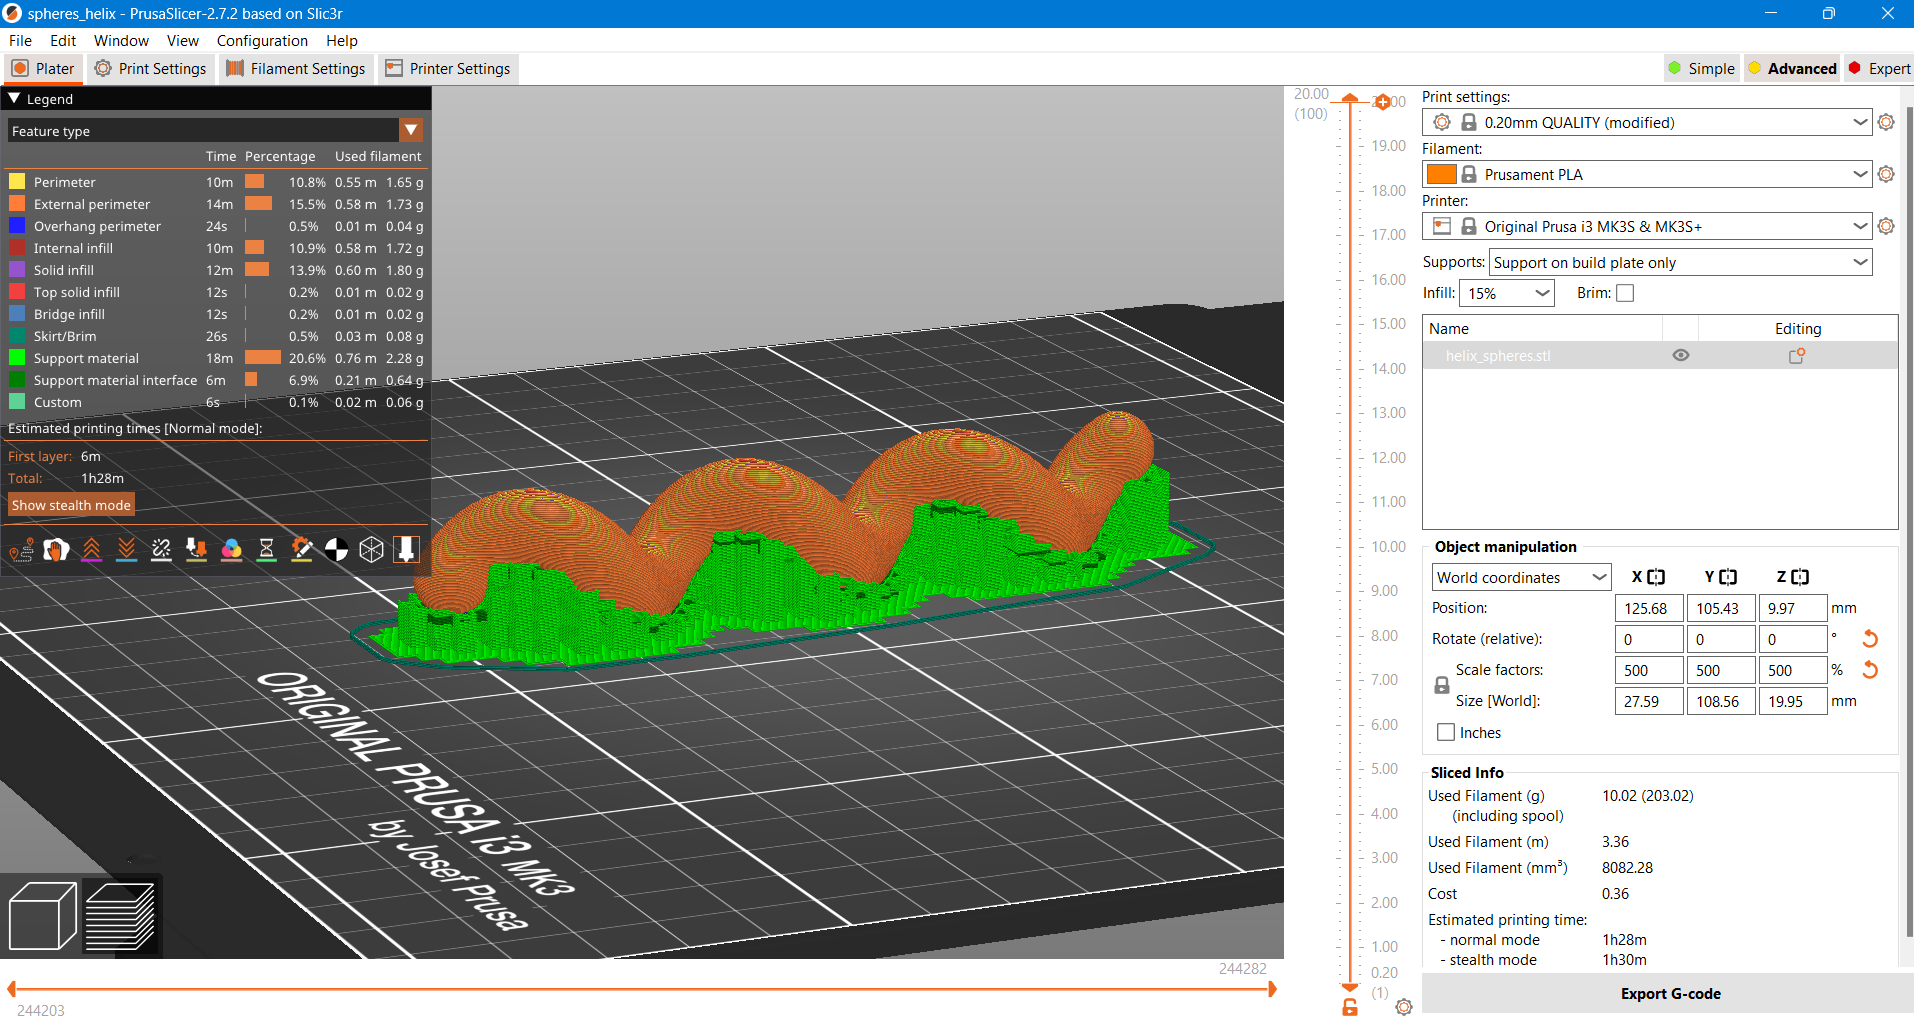
\includegraphics[width=\textwidth]{images/prusaslicer.png}
	\caption[Softvér PrusaSlicer.]{Slicing plochy v softvéri PrusaSlicer.}
	\label{fig:prusaslicer}
\end{figure}

\subsubsection{Parametre tlače}
Ako vstupný formát do PrusaSlicer-u sme používali \verb|.stl|. \\
Typ tlačiarne: Original Prusa i3 MK3S \& MK3S+ \\
Nastavenie tlače: 0.20mm QUALTY \\
Filament: Prusament PLA \\
Podpory: Podpora len na stavebnej doske \\
Infill: 15\% \\
Teplota trysky: 215\textdegree{}C \\
Teplota podložky: 60\textdegree{}C \\
Kvôli nefunkčnosti tlače z SD karty, sme pre 3D tlač používali počítač prepojený USB káblom s tlačiarňou. Počítač musel byť počas tlače neustále pripojený k tlačiarni a nesmel prejsť do režimu spánku, hibernácie alebo sa vypnúť. Prerušenie pripojenia k počítaču by malo za následok prerušenie tlače bez možnosti obnovenia tlače. 

\subsection{Pronterface}
Pronterface je jednoduché grafické používateľské rozhranie, ktoré používateľom ponúka možnosť monitorovať a ovládať tlačiareň z počítača pripojeného cez USB. Pomocou neho možno priamo pohybovať krokovými motormi, ovládať teplotu lôžka a trysky, posielať príkazy G-kódu priamo cez terminál alebo konzolové okno a mnoho ďalšieho. Pronterface je súčasťou balíka jednoduchých nástrojov Printrun na správu a ovládanie 3D tlačiarní aj CNC strojov. Napriek svojmu základne vyzerajúcemu dizajnu a zastaranej grafike zostáva užitočným nástrojom, ktorý si udržiava silnú pozíciu v komunite 3D tlačiarov \cite{Prontersetup}. 

Stiahli sme jeho poslednú veziu 2.0.1 na webovej lokalite \cite{Pronterface}. Pomocou Správcu zariadení systému Windows sme skontrolovali, ktorý port COM bol priradený našej 3D tlačiarni, bol to COM3. Po pripojení k tlačiarni sme zvolili tlačidlo Connect. Potom sme načítali model tlačidlom \verb|Load file| a vybrali súbor vo formáte \verb|.gcode|. V aplikácii sme skontrolovali nastavenú teplotu trysiek a podložky, aby zodpovedala zvolenému materiálu podľa našich pokynov. Po načítaní modelu sa v pravom stĺpci zobrazil pesimisticky odhad času tlače.

\begin{figure}[h]
	\centering
	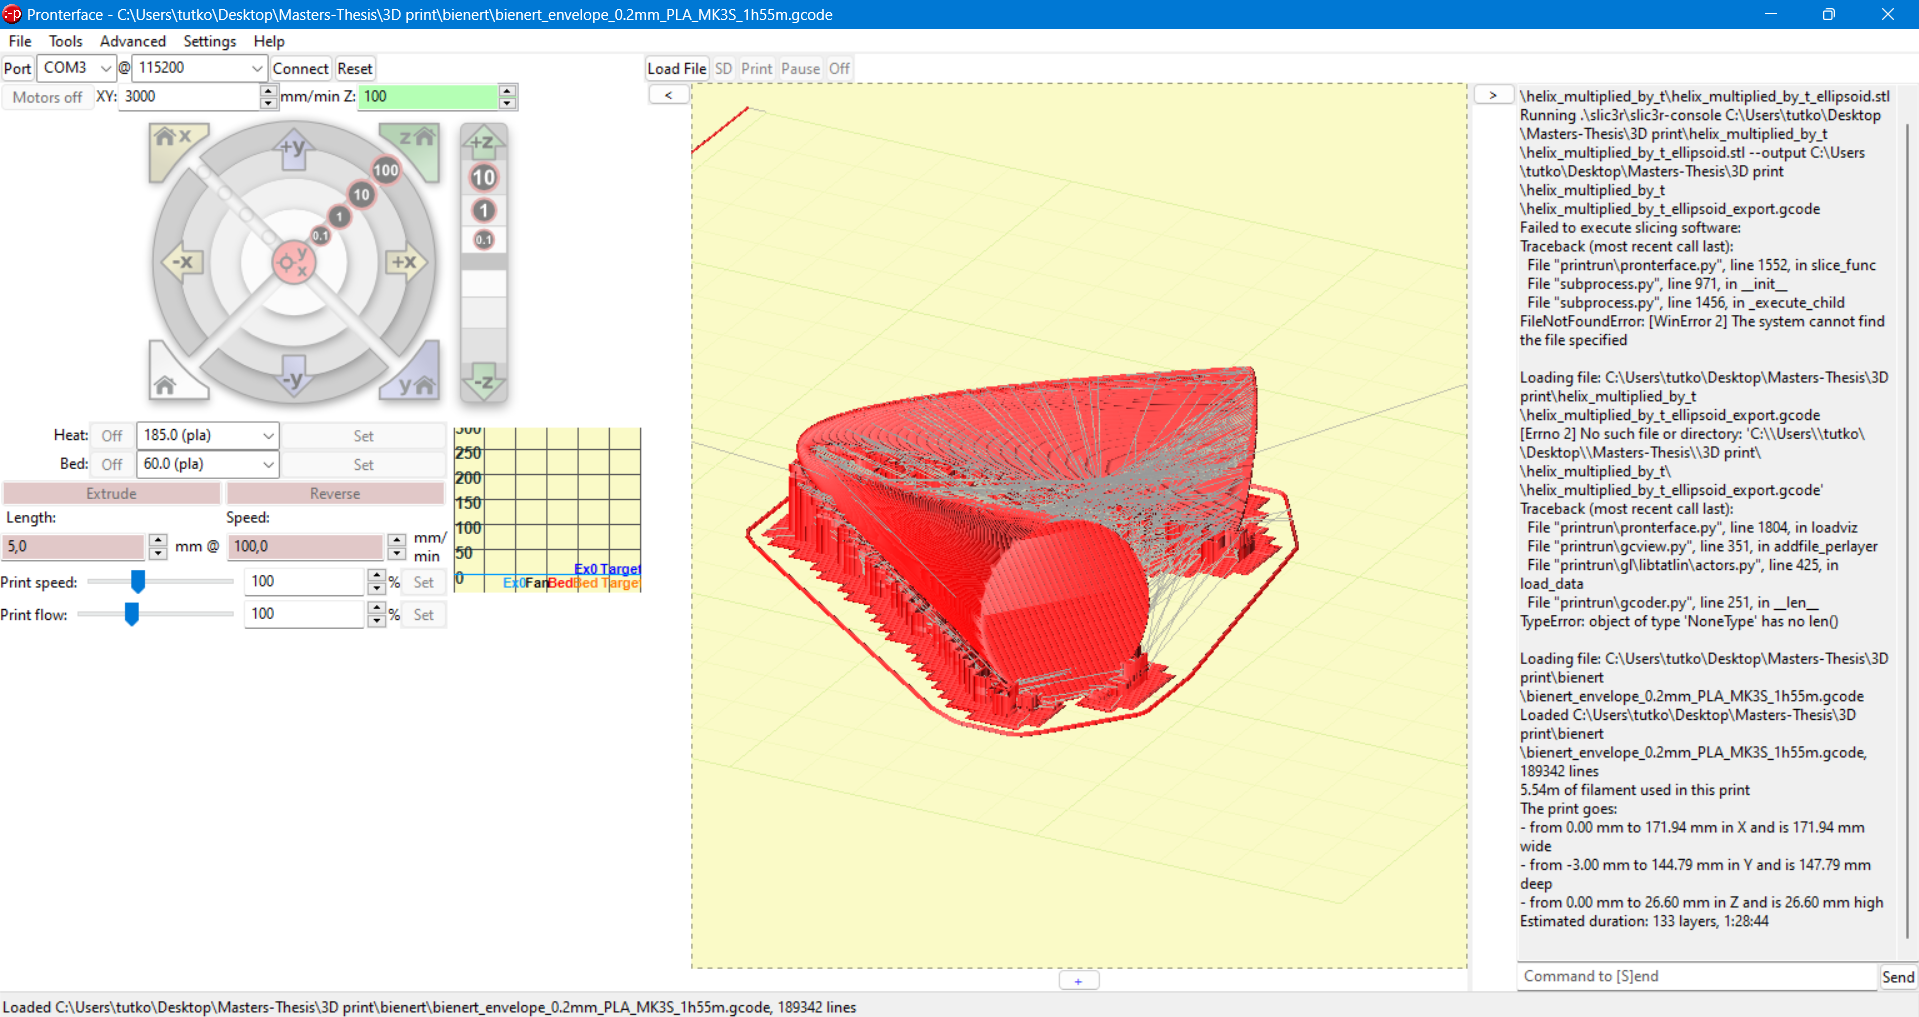
\includegraphics[width=\textwidth]{images/pronterface.png}
	\caption[Softvér Pronterface.]{Príprava na tlač plochy v softvéri Pronterface.}
	\label{fig:pronterface}
\end{figure}

\section{Zhrnutie procesu}
Najprv sme pripravili vstupné parametre v textovom súbore, ktorý sme načítali pred spustením skriptu. Python skript vygeneroval objekty v Blendri, kde bolo potrebné objekty vhodne pospájať a doplniť pletivo. Vytvorené plochy sme uzavreli a exportovali do programom PrusaSlicer podporovaného formátu, v našom prípade \verb|.stl|, ktorý pre plochy pripravil \verb|.gcode| na 3D tlač. Súbor \verb|.gcode| sa následne vložil na SD kartu alebo do softvéru Pronterface a mohli sme realizovať tlač po načítaní SD karty tlačiarňou alebo pripojení počítaču k tlačiarni.

\begin{figure}[h]
	\centering
	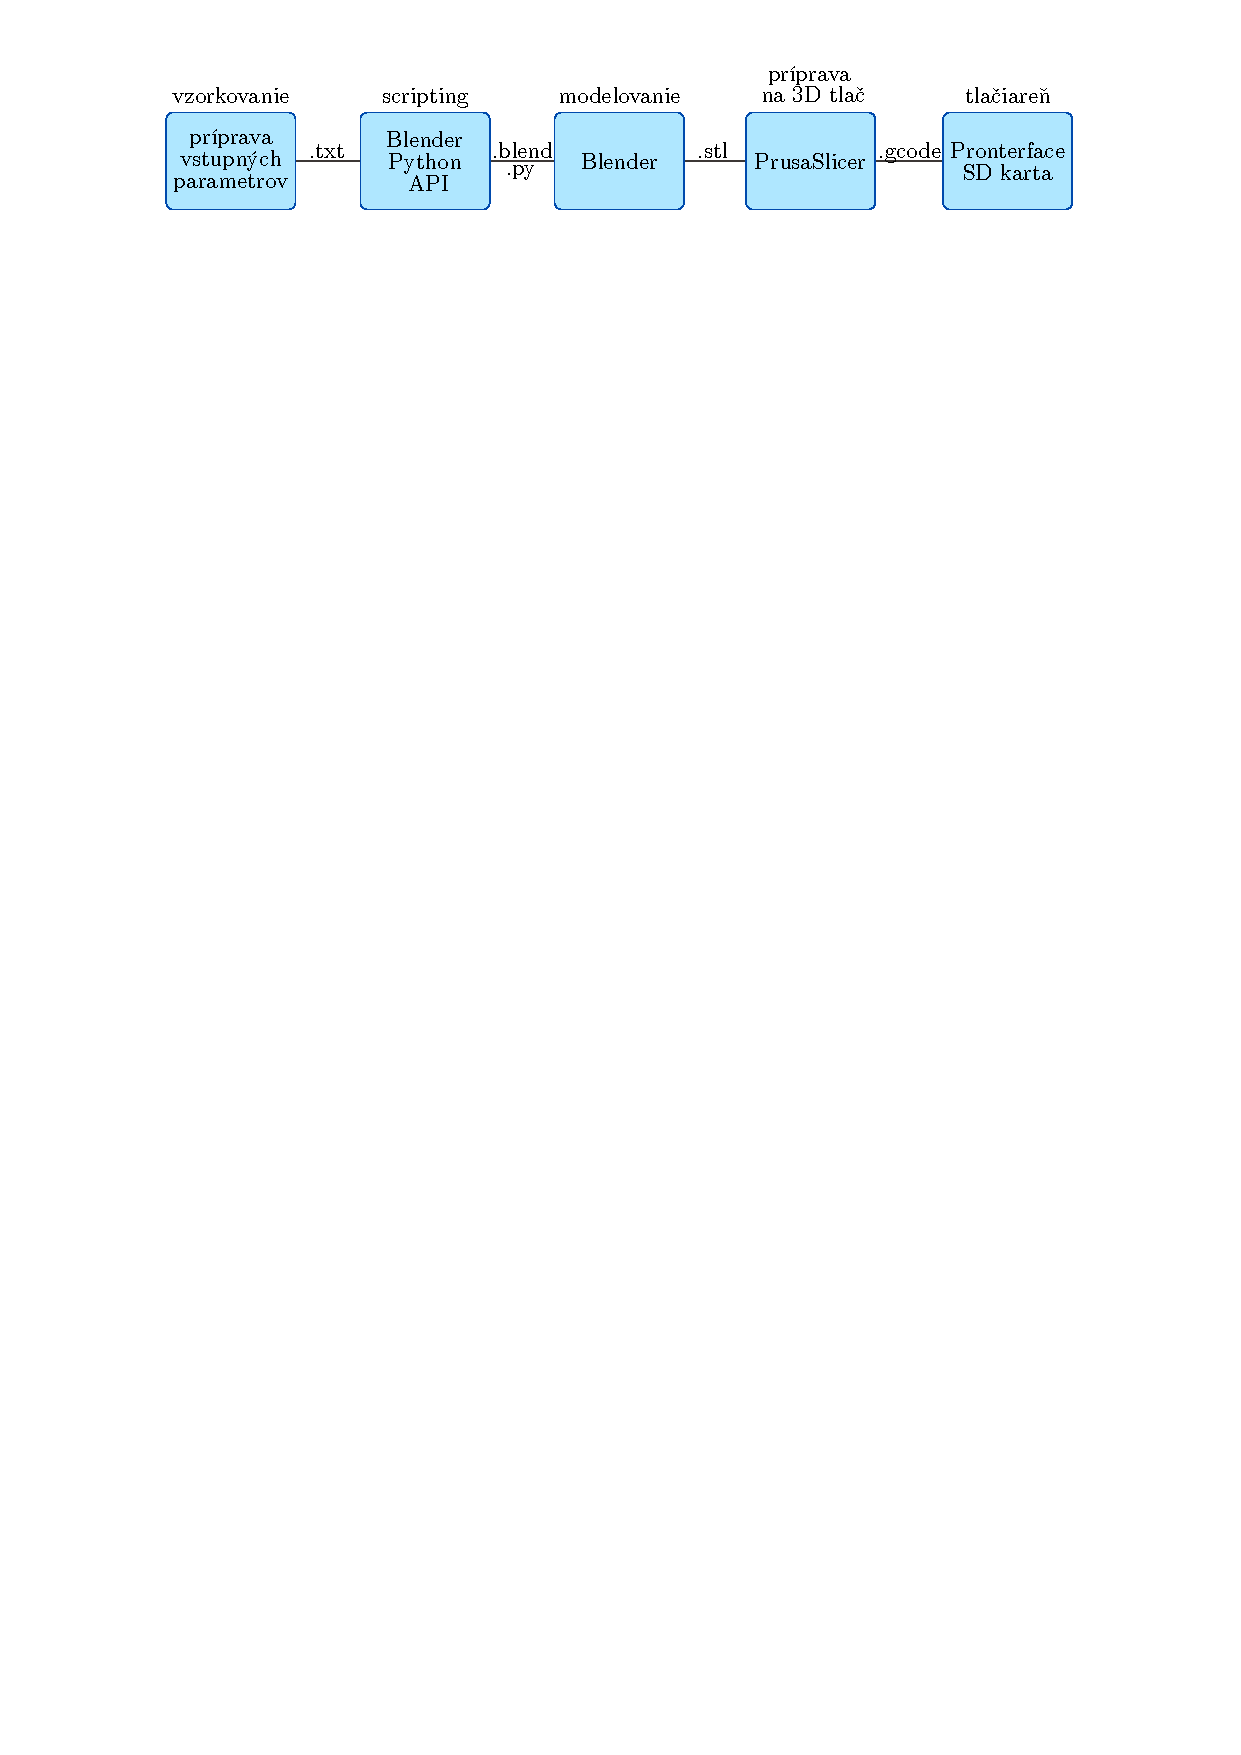
\includegraphics[trim={2.8cm 26cm 0cm 1cm},clip]{images/pipeline3.pdf}
	\caption[Schéma procesu od vstupu až po výstup.]{Schéma procesu.}
	\label{fig:pipeline}
\end{figure}
